
\documentclass[ letterpaper, titlepage, fleqn]{article}

\usepackage[utf8]{inputenc}
\usepackage[slovene]{babel}
\usepackage[margin=60px]{geometry}
\usepackage{amsmath}
\usepackage{amssymb}
\usepackage{enumerate}
\usepackage{graphicx}
\usepackage{mathrsfs}
\usepackage{mathabx}
\usepackage{faktor}
\usepackage{bbm}

\setlength\parindent{0pt}

\newcommand{\R}{\mathbb R}
\newcommand{\N}{\mathbb N}
\newcommand{\Z}{\mathbb Z}
\newcommand{\C}{\mathbb C}
\newcommand{\Q}{\mathbb Q}
\newcommand{\F}{\mathscr{F}}
\newcommand{\E}{\mathbb E}
\newcommand{\FF}{\mathbb F}
\newcommand{\K}{\mathbb K}
\newcommand{\D}{\mathbb D}
\newcommand{\J}{\mathscr J}
\newcommand{\T}{\mathscr T}

\newcommand{\mul}{\text{mul}}
\newcommand{\add}{\text{add}}
\newcommand{\abs}{\text{abs}}
\newcommand{\aph}{\text{@}}
\newcommand{\primea}{\textsc{\char13}}
\newcommand{\norm}[1]{\left\lVert#1\right\rVert}
\newcommand{\scalar}[1]{\left\langle#1\right\rangle}
\newcommand{\zeroradical}{\sqrt{0}}
\newcommand{\Bin}{\text{Bin}}
\newcommand{\id}{\text{id}}
\newcommand{\ind}{\mathbbm{1}}

\begin{document}

\section{1}

\subsection{}
Če zapišemo gostote v eksponentni obliki, dobimo
$$f(x; a,b) = \frac{b^a}{\Gamma(a)} e^{-\scalar{(a+1, b), (\ln(x), 1/x)}} \cdot \ind_{(0,\infty)}(x),$$
torej dobimo po Neuman-Fischerjevem faktorizacijskem izreku, da je
$$T(x) = (\ln(x), 1/x)$$
zadostna statistika za ta model.

\subsection{}
Ker smo v parametričnem modelu z zvezno odvedljivimi gostotami, lahko iščemo stacionarne točke gostot 
z logaritmično enačbo verjetja. Računamo
\begin{equation*}
\begin{aligned}
&l(a,b) := \ln(f(x; a,b)) = a\ln(b) - \ln(\Gamma(a)) - (a+1)\ln(x) - \frac{b}{x} \\
&\frac{\partial l}{\partial a}(a,b) = \ln(b) - \frac{\Gamma'(a)}{\Gamma(a)} - \ln(x) \\
&\frac{\partial l}{\partial b}(a,b) = \frac{a}{b} - \frac{1}{x}.
\end{aligned}
\end{equation*}
Zapišemo lahko logaritemsko enačbo verjetja
$$\ln(b) - \frac{\Gamma'(a)}{\Gamma(a)} - \ln(x) = \frac{a}{b} - \frac{1}{x} = 0,$$
iz česar takoj dobimo $b = ax$, za drugo enačbo pa potem sledi, da rešujemo
$$\Psi(a) := \ln(a) - \frac{\Gamma'(a)}{\Gamma(a)} = 0.$$
Po posledici Bernsteinovega izreka o monotonih funkcijah velja, da je za $x > 0$
$$\Psi(x) - \frac{1}{2x} > 0,$$
torej naša funkcija nima ničel in zato cenilka po metodi največjega verjetja ne obstaja (digamma wiki).

\subsection{}
Za $k\in\N$ velja
$$
m_k := P_{(a,b)}[\id^k] = \int_0^\infty \frac{b^a}{\Gamma(a)} x^{-a-1} e^{-b/x} x^k dx
= \frac{b^a}{\Gamma(a)} \frac{\Gamma(a-k)}{b^{a-k}} \int_0^\infty \frac{b^{a-k}}{\Gamma(a-k)} x^{-(a-k)-1} e^{-b/x} dx 
= b^k \frac{\Gamma(a-k)}{\Gamma(a)}.
$$
Označimo
\begin{equation*}
\begin{aligned}
&\hat{b}(x_1, x_2, x_3) := \left(\frac{x_1}{x_2} - \frac{x_2}{x_3}\right)^{-1} \\
&\hat{a}(x_1, x_2, x_3) := \frac{\hat{b}(x_1,x_2,x_3)}{x_1} + 1 \\
\end{aligned}
\end{equation*}
in opazimo, da je $\hat{b}(m_1,m_2,m_3) = b$ in $\hat{a}(m_1,m_2,m_3) = a$,
torej dobimo zaporedje cenilk po metodi momentov
$$(\hat{a}, \hat{b}) \circ (\hat{m_1^n}, \hat{m_2^n}, \hat{m_3^n}),$$
kjer je
$$\hat{m_k^n}(x) = \frac{1}{n} \sum_{i=1}^n x_i^ k.$$
Ker je $g = (\hat{a}, \hat{b})$ zvezna na $\R_+^3$, je ta cenilka dosledna. 
Sicer pa $g$ ni trivialna preslikava in zato ne moremo enostavno analizirati porazdelitve, 
niti nujno izračunati povprečne vrednosti.

\subsection{}
Naj bodo torej $X_i \sim P_\vartheta$ NEP. Definirajmo NEP vektorje $Y_i := (X_i, X_i^2, X_i^3)$ in označimo
$$
M_n := (\hat{m_1^n}, \hat{m_2^n}, \hat{m_3^n}) \quad \text{in} \quad
\hat{\vartheta}_n := g \circ M_n.
$$
Po centralnem limitnem izreku velja
$$\sqrt{n} \cdot \left(M_n(X_1, \dots, X_n) - \mu \right) = \sqrt{n} \cdot\left(\frac{1}{n} \sum_{i=1}^n Y_i - \mu\right) \xrightarrow[n\to\infty]{D} N(0, \Sigma),$$
kjer je $\mu$ pričakovana vrednost, $\Sigma$ pa variančno-kovariančna matrika vektorjev $Y_i$.
Potem nam metoda delta skupaj s Cramer-Woldovim pravilom zagotovi
$$\sqrt{n} \cdot (\hat{\vartheta}_n(X_1, \dots, X_n) - \vartheta) = \sqrt{n} \cdot (g(M_n(X_1, \dots, X_n)) - g(\mu)) \xrightarrow[n\to\infty]{D} N(0, \J_g(\mu) \Sigma \J_g(\mu)^T),$$
saj je očitno $\mu = [m_1, m_2, m_3]^T$.

\subsection{}
Enostavno izračunamo
$$\Sigma = 
\begin{bmatrix}
m_2 - m_1^2 & m_3 - m_1m_2 & m_4 - m_1m_3 \\
m_3 - m_1m_2 & m_4 - m_2^2 & m_5 - m_2m_3 \\
m_4 - m_1m_3 & m_5 - m_2m_3 & m_6 - m_3^2 
\end{bmatrix}
$$
in označimo
$$A := \J_g(\mu) \Sigma \J_g(\mu)^T.$$
Definirajmo sedaj zaporedje cenilk $\hat{A}_n$ tako, da zamenjamo v $A$  elemente $m_i$ z $\hat{m_i^n}$.
Potem uporabimo Sluckyjev izrek in zveznost korena ter inverza spd matrike, da dobimo
$$\pi_n(X_1, \dots, X_n, \vartheta) := \sqrt{n} \cdot \hat{A}_n^{-1/2} \left(\hat{\vartheta}_n(X_1, \dots, X_n) - \vartheta\right) \xrightarrow[n\to\infty]{D} N(0, I).$$
Naj bo $B \subset \R^2$ neka množica, ki zadošča
$$P(\pi_n(X_1, \dots, X_n, \vartheta) \in B) \approx N(0,I)(B) = 1 - \alpha,$$
Sledi
$$P(\pi_n(X_1, \dots, X_n, \vartheta) \in B) = P(\hat{\vartheta}_n(X_1, \dots, X_n) - \vartheta \in \hat{A}_n^{1/2}\left(B\right) / \sqrt{n}) = P(\vartheta \in \hat{\vartheta}_n(X_1, \dots, X_n) - \hat{A}_n^{1/2}\left(B\right) / \sqrt{n}),$$
torej je območje zaupanja za $\vartheta$ enako
$$\hat{\vartheta}_n(X_1, \dots, X_n) - \hat{A}_n^{1/2}\left(B\right) / \sqrt{n}.$$
Vprašanje izbire množice $B$ lahko rešimo s predpostavko, da je to zaprta krogla s središčem v $0$ v neki normirani metriki, 
s čimer se verjetno da dokazati enoličnost njenega radija.


\section{2}
Naj bodo $X_i \sim P_\mu$ NEP. Po Rao-Blackwellevem izreku lahko najdemo NCEND kot pogojno upanje 
nepristranske cenilke $\ind_{\{X_1 \leq 5\}}$  pogojno na kompletno in zadostno statistiko
$$\bar{X}^n = \frac{1}{n} \sum_{i=1}^n X_i.$$
Označimo $Y = \bar{X}^n - \mu$ in definirajmo
$$\tilde{X} = X_1 - \zeta Y, \text{ kjer je } \zeta = P[X_1Y] / \sigma(Y)^2.$$
Zanjo velja
$$P[\tilde{X}Y] = P[X_1Y] - \zeta P[Y^2] = 0,$$
torej sta $\tilde{X}$ in $Y$ nekorelirani, ker pa sta normalni, sta tudi neodvisni. 
Sedaj lahko zapišemo
\begin{equation*}
\begin{aligned}
P[\ind_{\{X_1 \leq 5\}} \mid \bar{X}^n = t] &= P(X_1 \leq 5 \mid \bar{X}^n = t) 
= P(\tilde{X} + \zeta Y \leq 5 \mid Y + \mu = t) = P(\tilde{X} + \zeta (t - \mu) \leq 5) \\
&= P(X_1 - \zeta (\bar{X}^n - \mu) + \zeta(t - \mu) \leq 5) = P(X_1 - \zeta \bar{X}^n \leq 5 + \zeta t).
\end{aligned}
\end{equation*}
Konkretno:
$$P[X_1Y] = P[(\sigma Z_1 + \mu)Y] = P[\sigma Z_1 Y] = P[\sigma Z_1 \sum_{i=1}^n \frac{\sigma}{n} Z_i] = \frac{\sigma^2}{n} P[Z_1^2]  = \frac{\sigma^2}{n},$$
torej skupaj z dejstvom $\sigma(Y) = \frac{\sigma}{\sqrt{n}}$ dobimo $\zeta = 1$ in zaporedje cenilk
$$U_n(\bar{x}^n) = P(\sigma (1 + 1/\sqrt{n})Z \leq 5 + \bar{x}^n) = \Phi\left(\frac{5 + \bar{x}^n}{\sigma(1 + 1/\sqrt{n})}\right)$$


\section{3}
\subsection{}
Ker je
$$
f(k; \vartheta) = -\frac{\vartheta^k}{k\ln(1-\vartheta)} = -\frac{e^{k\ln(\vartheta)}}{k\ln(1-\vartheta)} \implies 
f(k_1, \dots, k_n; \vartheta) = (-\ln(1-\vartheta))^{-n} \prod_{i=1}^n k_i^{-1} e^{\ln(\vartheta) \sum_{i=1}^n k_i}
$$
in $\ln((0,1))  = (-\infty, 0) \in \T_{EVK} \smallsetminus \{\emptyset\}$, je to eksponentni model s polnim rangom, 
torej je statistika 
$$T_n(k_1, \dots, k_n) = \sum_{i=1}^n k_i$$
kompletna zadostna.

\subsection{}
Ker imamo eksponenten model s funkcijo $Q = \ln$, ki je strogo naraščajoča na $(0,1)$, lahko uporabimo Neuman-Pearsonovo
lemo za konstrukcijo enakomerno najmočnejših randomiziranih preizkusov. 
Ker ima model druge momente si lahko pomagamo tudi z normalnimi aproksimacijami (ali asimptotično normalnostjo).

\subsection{}
Poskušajmo postopati z Neuman-Pearsonovo lemo. Označimo torej $\vartheta_0 = 0.7$ in $\alpha = 0.05$.
Potem imamo enakomerno najmočnejši randomiziran preizkus za $\vartheta \leq \vartheta_0$ proti alternativi
$\vartheta \ge \vartheta_0$ v obliki
$$
\phi(k_1, \dots, k_n)= 
\begin{cases}
1 \mid & T_n(k_1, \dots, k_n) > C \\
\gamma \mid &  T_n(k_1, \dots, k_n) = C \\
0 \mid &  T_n(k_1, \dots, k_n) < C
\end{cases},
$$
kjer določimo $C \in\N$ in $\gamma \in [0,1)$ enolično s pogojem
$$\beta(\vartheta_0) = P_{\vartheta_0}[\Phi] = P_{\vartheta_0}(T_n > C) + \gamma P_{\vartheta_0}(T_n = C) = \alpha.$$
Idealno bi bilo imeti porazdelitev $T_n$, a ta vključuje izračun vsot, ki v splošnem nimajo zaključene oblike ($\sum_{k=1}^d \vartheta^k / k$). Če bi imeli dovolj majhen vzorec, to tudi ne bi bil problem, saj bi izračunali posamezne vrednosti gostote $T_n$ z brute-force varianto. Ker pa je vzorec velikosti $n=100$ relativno velik, tega ne moremo izvesti. Lahko pa zato $T_n$ aproksimiramo z normalno porazdelitvijo (po CLI). Računamo
\begin{equation*}
\begin{aligned}
\mu_\vartheta 
&:= P_{\vartheta}[\id] 
= -\frac{1}{\ln(1 - \vartheta)} \sum_{k\in\N} \vartheta^k 
= -\frac{\vartheta}{(1 - \vartheta)} \frac{1}{\ln(1 - \vartheta)} \\
\sigma_\vartheta^2 
&:= V_{\vartheta}[\id] 
= P_{\vartheta}[\id^2] - P_{\vartheta}[\id]^2 
= -\frac{1}{\ln(1 - \vartheta)} \sum_{k\in\N} k\vartheta^k - \mu_\vartheta^2 
= -\frac{1}{\ln(1 - \vartheta)} \frac{\vartheta}{(1-\vartheta)^2} - \mu_\vartheta^2.
\end{aligned}
\end{equation*}
Označimo NEP model
$$\tilde{P}_\vartheta := N(\mu_\vartheta, \sigma_\vartheta^2)^{\times n}.$$
Sedaj lahko ocenimo gostoto statistike $T_n$ kot
$$P_\vartheta(T_n = k) \approx \tilde{P}_\vartheta(T_n \leq k) - \tilde{P}_\vartheta(T_n \leq k-1).$$
Aproksimirajmo:
\begin{equation*}
\begin{aligned}
\alpha &= 1 - P_{\vartheta_0}(T_n \leq C) + \gamma P_{\vartheta_0}(T_n = C) \\
&\approx 1 - \tilde{P}_{\vartheta_0}(T_n \leq C) + \gamma \tilde{P}_{\vartheta_0}(T_n \in [C-1, C]) \\
&= 1 - \Phi\left(\frac{C/n - \mu_{\vartheta_0}}{\sigma_{\vartheta_0} / \sqrt{n}}\right) + \gamma\left(
\Phi\left(\frac{C/n - \mu_{\vartheta_0}}{\sigma_{\vartheta_0} / \sqrt{n}}\right) -
\Phi\left(\frac{(C-1)/n - \mu_{\vartheta_0}}{\sigma_{\vartheta_0} / \sqrt{n}}\right)
\right).
\end{aligned}
\end{equation*}
Vzamemo prvi $C\in\N$, za katerega je 
$$\gamma = \frac{\alpha +
\Phi\left(\frac{C/n - \mu_{\vartheta_0}}{\sigma_{\vartheta_0} / \sqrt{n}}\right) - 1}
{\Phi\left(\frac{C/n - \mu_{\vartheta_0}}{\sigma_{\vartheta_0} / \sqrt{n}}\right) -
\Phi\left(\frac{(C-1)/n - \mu_{\vartheta_0}}{\sigma_{\vartheta_0} / \sqrt{n}}\right)} \in [0,1).$$
Dobimo $C = 221$ in $\gamma \approx 0.143$. Na spodnji sliki je funkcija moči, kjer so spet vse vrednosti aproksimirane z normalno porazdelitvijo.
\begin{center}
\begin{figure}[h]
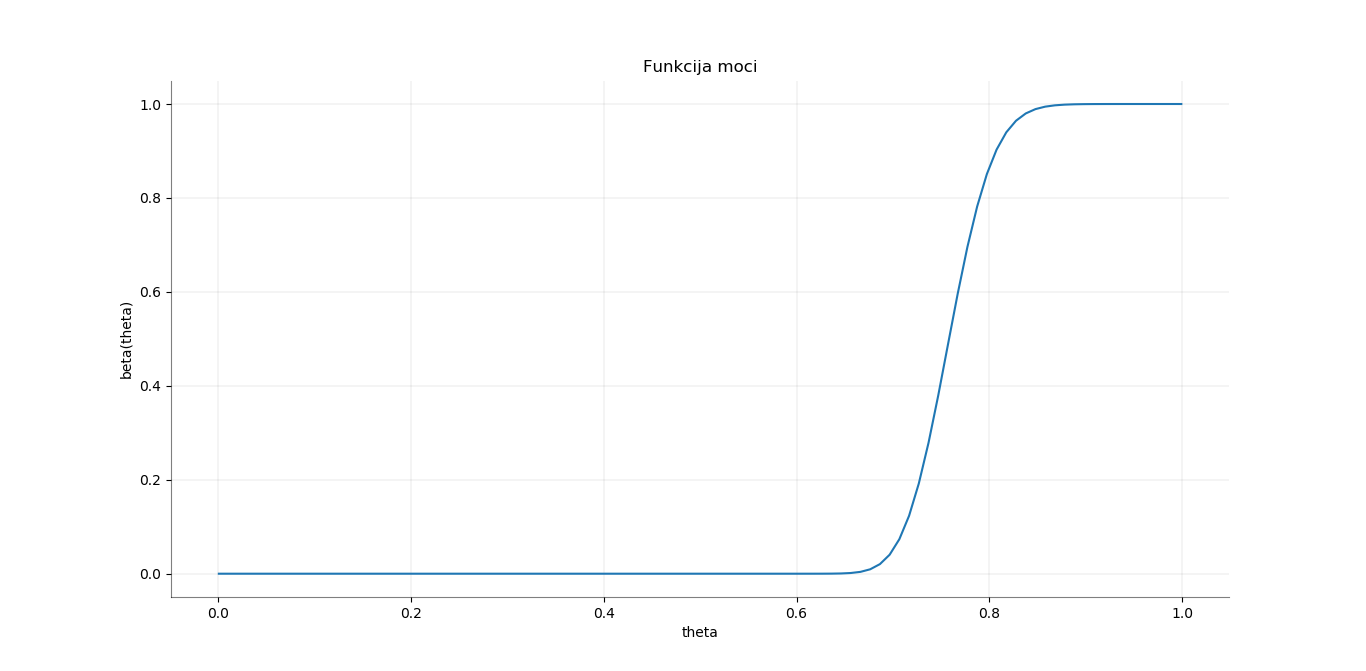
\includegraphics[width=18cm]{graphics/FunkcijaMoci.png}
\caption{Funkcija moči dobljenega testa.}
\end{figure}
\end{center}

\section{}
\subsection{}
Označimo spet
$$T(x_1, \dots, x_n) = \sum_{i=1}^n x_i.$$
Neuman-Pearsonov test za hipotezo $p = p_0$ proti alternativi ima obliko
$$
\phi(x)= 
\begin{cases}
1 &\mid T(x) \in (C_1(p_0), C_2(p_0)) \\
\gamma_j(p_0)  &\mid  T(x) = C_j(p_0) \\
0 &\mid  T(x) \notin [C_1(p_0), C_2(p_0)]
\end{cases},
$$
kjer so vrednosti $C_j(p_0)$, $\gamma_j(p_0)$ določene z zahtevo
$$P_{p_0}[\phi_{p_0}] = \alpha \quad \text{in} \quad \frac{d}{dp_0} P_{p_0}[\phi_{p_0}] = 0.$$
Izračunamo 
\begin{equation*}
\begin{aligned}
P_{p_0}[\phi_{p_0}] &= P_{p_0}(T< C_1(p_0)) + P_{p_0}(T > C_2(p_0)) 
+ \gamma_1(p_0) P_{p_0}(T = C_1(p_0)) + \gamma_2(p_0) P_{p_0}(T = C_2(p_0)) \\
&= 1 - \sum_{i=C_1(p_0)}^{C_2(p_0)} \binom{n}{i} p_0^i (1-p_0)^{n-i}
+ \sum_{i\in\{1,2\}} \gamma_i(p_0) \binom{n}{C_i(p_0)} p_0^{C_i(p_0)} (1-p_0)^{n -C_i(p_0)}
\end{aligned}
\end{equation*}
in
\begin{equation*}
\begin{aligned}
\frac{d}{dp_0} P_{p_0}[\phi_{p_0}] &= 
- \sum_{i=C_1(p_0)}^{C_2(p_0)} \binom{n}{i}\left(i p_0^{i-1} (1-p_0)^{n-i} - (n-i) p_0^i (1-p_0)^{n-i-1}\right) \\
&\quad + \sum_{i\in\{1,2\}} \gamma_i(p_0) \binom{n}{C_i(p_0)} \left(C_i(p_0) p_0^{C_i(p_0-1)} (1-p_0)^{n -C_i(p_0)} -
(n-C_i(p_0)) p_0^{C_i(p_0-1)} (1-p_0)^{n-C_i(p_0)-1}\right).
\end{aligned}
\end{equation*}
Če privzamemo, da so vse vrednosti razen $\gamma_i(p_0)$ konstantne, je to sistem dveh linearnih enačb za $\gamma_i(p_0)$.
To, da so ostale stvari konstantne dosežemo tako, da testiramo vsak $C_1(p_0) \in \{0,\dots,n-1\}$ in $C_2(p_0) \in \{C_1(p_0)+1,\dots,n\}$ posebej. Vzamemo prve vrednosti, pri katerih velja $0 \leq \gamma_i(p_0) \leq 1$ za $i=1,2$.
\begin{center}
\begin{figure}[h]
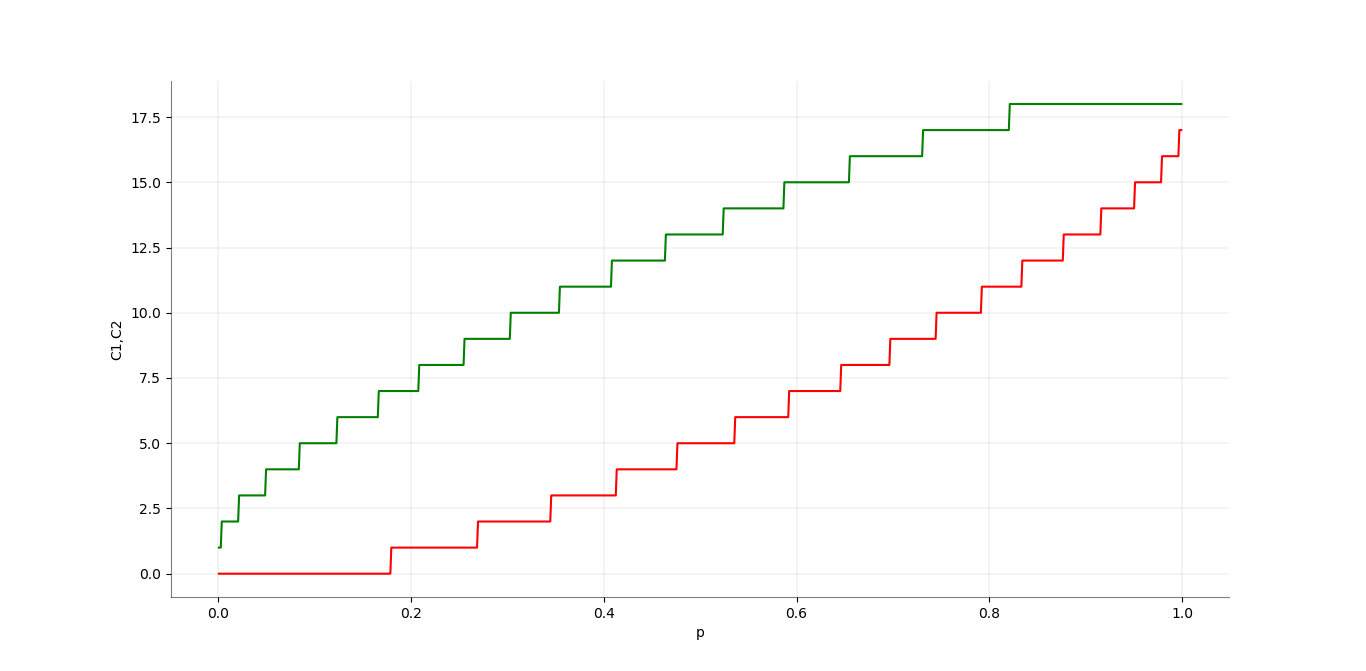
\includegraphics[width=18cm]{graphics/C1C2.png}
\caption{$C_1(p)$ in $C_2(p)$  na diskretizaciji $(0,1)$ na $1000$ točkah.}
\end{figure}
\end{center}

Za interval zaupanja definiramo
$$I(T(x)) := \{p \in (0,1) \mid \phi_p(x) < 1\} = \{p \in (0,1) \mid T(x) \in [C_1(p), C_2(p)]\}.$$
Za vsak $k=0,1,\dots,n$ bomo vzeli vse $p$ na neki diskretizaciji $(0,1)$, ki so v $I(k)$. Spodnja tabela prikazuje aproksimacijo $I\circ T$ pri delitvi intervala (0,1) na $1000$ delov, z zaokrožitvijo krajišč intervala na $4$ decimalna mesta.

\begin{center}
\begin{tabular}{ l | l }
k & I(k) \\
\hline
0 & (0, 0.1798] \\
1 & (0, 0.2697] \\
2 & [0.004, 0.3457] \\
3 & [0.022, 0.4136] \\
4 & [0.0499, 0.4765] \\
5 & [0.0849, 0.5365] \\
6 & [0.1239, 0.5924] \\
7 & [0.1668, 0.6464] \\
8 & [0.2088, 0.6973] \\
9 & [0.2557, 0.7453] \\
10 & [0.3037, 0.7922] \\
11 & [0.3546, 0.8342] \\
12 & [0.4086, 0.8771] \\
13 & [0.4645, 0.9161] \\
14 & [0.5245, 0.951] \\
15 & [0.5874, 0.979] \\
16 & [0.6553, 0.997] \\
17 & [0.7313, 1) \\
18 & [0.8212, 1) \\
\end{tabular}
\end{center}

\subsection{}
Zaokroženo na $4$ decimalna mesta dobimo
$$\gamma_1(0.72) \approx 0.1787 \quad \text{in} \quad \gamma_2(0.72) \approx 0.6852.$$

\subsection{}
Ocena minimuma vrednosti na spodnjem grafu je $0.9550165005548836$, kar je ocena za koeficient zaupanja.
\begin{center}
\begin{figure}[h]
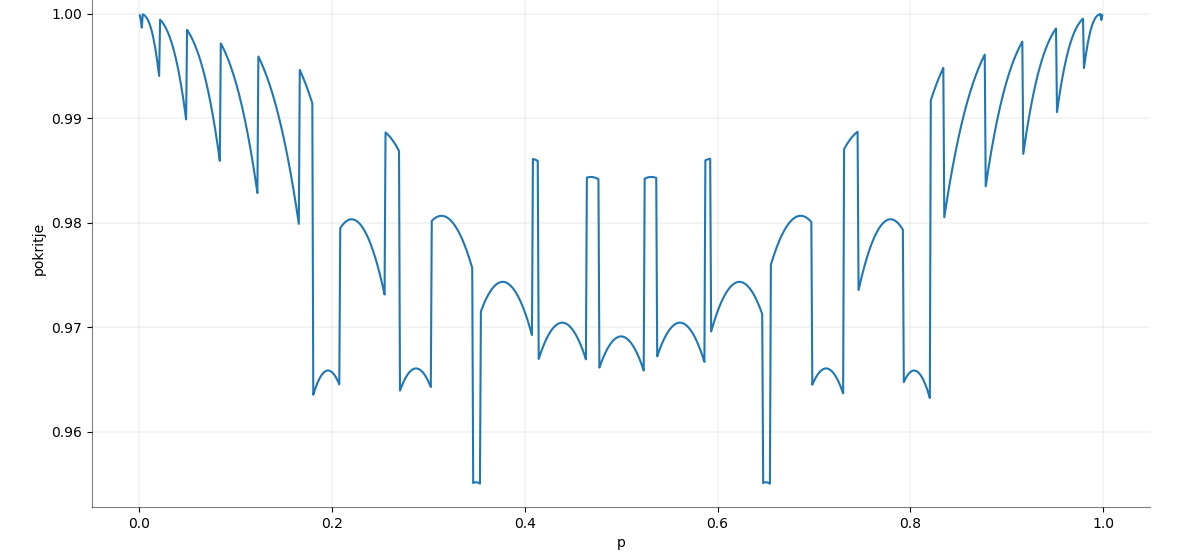
\includegraphics[width=18cm]{graphics/Pokritje.png}
\end{figure}
\end{center}

\subsection{}
Program nam vrne
\begin{equation*}
\begin{aligned}
C_1 = 15 \quad &\text{in} \quad C_2 = 24 \\
\gamma_1 \approx 0.6922 \quad &\text{in} \quad \gamma_2 \approx 0.0029
\end{aligned}
\end{equation*}


\end{document}